\documentclass[twoside]{book}

% Packages required by doxygen
\usepackage{fixltx2e}
\usepackage{calc}
\usepackage{doxygen}
\usepackage[export]{adjustbox} % also loads graphicx
\usepackage{graphicx}
\usepackage[utf8]{inputenc}
\usepackage{makeidx}
\usepackage{multicol}
\usepackage{multirow}
\PassOptionsToPackage{warn}{textcomp}
\usepackage{textcomp}
\usepackage[nointegrals]{wasysym}
\usepackage[table]{xcolor}

% Font selection
\usepackage[T1]{fontenc}
\usepackage[scaled=.90]{helvet}
\usepackage{courier}
\usepackage{amssymb}
\usepackage{sectsty}
\renewcommand{\familydefault}{\sfdefault}
\allsectionsfont{%
  \fontseries{bc}\selectfont%
  \color{darkgray}%
}
\renewcommand{\DoxyLabelFont}{%
  \fontseries{bc}\selectfont%
  \color{darkgray}%
}
\newcommand{\+}{\discretionary{\mbox{\scriptsize$\hookleftarrow$}}{}{}}

% Page & text layout
\usepackage{geometry}
\geometry{%
  a4paper,%
  top=2.5cm,%
  bottom=2.5cm,%
  left=2.5cm,%
  right=2.5cm%
}
\tolerance=750
\hfuzz=15pt
\hbadness=750
\setlength{\emergencystretch}{15pt}
\setlength{\parindent}{0cm}
\setlength{\parskip}{3ex plus 2ex minus 2ex}
\makeatletter
\renewcommand{\paragraph}{%
  \@startsection{paragraph}{4}{0ex}{-1.0ex}{1.0ex}{%
    \normalfont\normalsize\bfseries\SS@parafont%
  }%
}
\renewcommand{\subparagraph}{%
  \@startsection{subparagraph}{5}{0ex}{-1.0ex}{1.0ex}{%
    \normalfont\normalsize\bfseries\SS@subparafont%
  }%
}
\makeatother

% Headers & footers
\usepackage{fancyhdr}
\pagestyle{fancyplain}
\fancyhead[LE]{\fancyplain{}{\bfseries\thepage}}
\fancyhead[CE]{\fancyplain{}{}}
\fancyhead[RE]{\fancyplain{}{\bfseries\leftmark}}
\fancyhead[LO]{\fancyplain{}{\bfseries\rightmark}}
\fancyhead[CO]{\fancyplain{}{}}
\fancyhead[RO]{\fancyplain{}{\bfseries\thepage}}
\fancyfoot[LE]{\fancyplain{}{}}
\fancyfoot[CE]{\fancyplain{}{}}
\fancyfoot[RE]{\fancyplain{}{\bfseries\scriptsize Generated by Doxygen }}
\fancyfoot[LO]{\fancyplain{}{\bfseries\scriptsize Generated by Doxygen }}
\fancyfoot[CO]{\fancyplain{}{}}
\fancyfoot[RO]{\fancyplain{}{}}
\renewcommand{\footrulewidth}{0.4pt}
\renewcommand{\chaptermark}[1]{%
  \markboth{#1}{}%
}
\renewcommand{\sectionmark}[1]{%
  \markright{\thesection\ #1}%
}

% Indices & bibliography
\usepackage{natbib}
\usepackage[titles]{tocloft}
\setcounter{tocdepth}{3}
\setcounter{secnumdepth}{5}
\makeindex

% Hyperlinks (required, but should be loaded last)
\usepackage{ifpdf}
\ifpdf
  \usepackage[pdftex,pagebackref=true]{hyperref}
\else
  \usepackage[ps2pdf,pagebackref=true]{hyperref}
\fi
\hypersetup{%
  colorlinks=true,%
  linkcolor=blue,%
  citecolor=blue,%
  unicode%
}

% Custom commands
\newcommand{\clearemptydoublepage}{%
  \newpage{\pagestyle{empty}\cleardoublepage}%
}

\usepackage{caption}
\captionsetup{labelsep=space,justification=centering,font={bf},singlelinecheck=off,skip=4pt,position=top}

%===== C O N T E N T S =====

\begin{document}

% Titlepage & ToC
\hypersetup{pageanchor=false,
             bookmarksnumbered=true,
             pdfencoding=unicode
            }
\pagenumbering{roman}
\begin{titlepage}
\vspace*{7cm}
\begin{center}%
{\Large My Project }\\
\vspace*{1cm}
{\large Generated by Doxygen 1.8.11}\\
\end{center}
\end{titlepage}
\clearemptydoublepage
\tableofcontents
\clearemptydoublepage
\pagenumbering{arabic}
\hypersetup{pageanchor=true}

%--- Begin generated contents ---
\chapter{Class Index}
\section{Class List}
Here are the classes, structs, unions and interfaces with brief descriptions\+:\begin{DoxyCompactList}
\item\contentsline{section}{\hyperlink{structnode}{node} }{\pageref{structnode}}{}
\item\contentsline{section}{\hyperlink{structnode1}{node1} }{\pageref{structnode1}}{}
\item\contentsline{section}{\hyperlink{structnode__info}{node\+\_\+info} }{\pageref{structnode__info}}{}
\end{DoxyCompactList}

\chapter{File Index}
\section{File List}
Here is a list of all files with brief descriptions\+:\begin{DoxyCompactList}
\item\contentsline{section}{\hyperlink{Lab1_8c}{Lab1.\+c} }{\pageref{Lab1_8c}}{}
\end{DoxyCompactList}

\chapter{Class Documentation}
\hypertarget{classAuthor}{}\section{Author Class Reference}
\label{classAuthor}\index{Author@{Author}}


{\ttfamily \#include $<$Author.\+h$>$}

\subsection*{Public Member Functions}
\begin{DoxyCompactItemize}
\item 
\hyperlink{classAuthor_a8873fad1ccf89e11a9f499d8a0e2607f}{Author} (const std\+::string \&\hyperlink{classAuthor_a618f8527df84dc680f62a967f6f5e96e}{name}, const std\+::string \&\hyperlink{classAuthor_a8542e2f9c1f481b40665cb3b32f43c8e}{email}, char \hyperlink{classAuthor_a3e7bac289b21d7f97dc2bf14e56b9a14}{gender})
\item 
std\+::string \hyperlink{classAuthor_a2d27943db18f822be1a301bca65fb6ef}{get\+Name} () const 
\item 
std\+::string \hyperlink{classAuthor_af7dd4e055b1a7ea0cf1623c1c0b46d62}{get\+Email} () const 
\item 
void \hyperlink{classAuthor_a3cf04f59de5f1f6cfb50a55667844cfd}{set\+Email} (const std\+::string \&\hyperlink{classAuthor_a8542e2f9c1f481b40665cb3b32f43c8e}{email})
\item 
char \hyperlink{classAuthor_a4ff6cc39d18894b0538e10a8e7170988}{get\+Gender} () const 
\item 
void \hyperlink{classAuthor_a5d5d6296cd6cf5c5017fc2f27a8f6925}{print} () const 
\end{DoxyCompactItemize}
\subsection*{Private Attributes}
\begin{DoxyCompactItemize}
\item 
std\+::string \hyperlink{classAuthor_a618f8527df84dc680f62a967f6f5e96e}{name}
\item 
std\+::string \hyperlink{classAuthor_a8542e2f9c1f481b40665cb3b32f43c8e}{email}
\item 
char \hyperlink{classAuthor_a3e7bac289b21d7f97dc2bf14e56b9a14}{gender}
\end{DoxyCompactItemize}


\subsection{Constructor \& Destructor Documentation}
\index{Author@{Author}!Author@{Author}}
\index{Author@{Author}!Author@{Author}}
\subsubsection[{\texorpdfstring{Author(const std\+::string \&name, const std\+::string \&email, char gender)}{Author(const std::string &name, const std::string &email, char gender)}}]{\setlength{\rightskip}{0pt plus 5cm}Author\+::\+Author (
\begin{DoxyParamCaption}
\item[{const std\+::string \&}]{name, }
\item[{const std\+::string \&}]{email, }
\item[{char}]{gender}
\end{DoxyParamCaption}
)}\hypertarget{classAuthor_a8873fad1ccf89e11a9f499d8a0e2607f}{}\label{classAuthor_a8873fad1ccf89e11a9f499d8a0e2607f}

\begin{DoxyCode}
7                                                                      : \hyperlink{classAuthor_a618f8527df84dc680f62a967f6f5e96e}{name}(
      \hyperlink{classAuthor_a618f8527df84dc680f62a967f6f5e96e}{name}) \{
8    \hyperlink{classAuthor_a3cf04f59de5f1f6cfb50a55667844cfd}{setEmail}(\hyperlink{classAuthor_a8542e2f9c1f481b40665cb3b32f43c8e}{email});  \textcolor{comment}{// Call setter to check for valid email}
9    \textcolor{keywordflow}{if} (\hyperlink{classAuthor_a3e7bac289b21d7f97dc2bf14e56b9a14}{gender} == \textcolor{charliteral}{'m'} || \hyperlink{classAuthor_a3e7bac289b21d7f97dc2bf14e56b9a14}{gender} == \textcolor{charliteral}{'f'}) \{
10       this->\hyperlink{classAuthor_a3e7bac289b21d7f97dc2bf14e56b9a14}{gender} = \hyperlink{classAuthor_a3e7bac289b21d7f97dc2bf14e56b9a14}{gender};
11    \} \textcolor{keywordflow}{else} \{
12       cout << \textcolor{stringliteral}{"Invalid gender! Set to 'u' (unknown)."} << endl;
13       this->\hyperlink{classAuthor_a3e7bac289b21d7f97dc2bf14e56b9a14}{gender} = \textcolor{charliteral}{'u'};
14    \}
15 \}
\end{DoxyCode}


Here is the call graph for this function\+:
\nopagebreak
\begin{figure}[H]
\begin{center}
\leavevmode
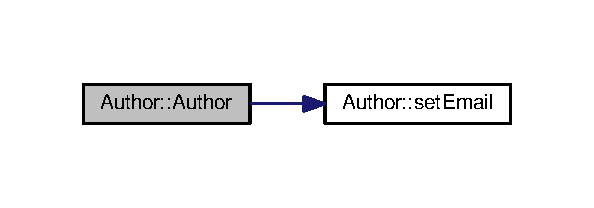
\includegraphics[width=285pt]{classAuthor_a8873fad1ccf89e11a9f499d8a0e2607f_cgraph}
\end{center}
\end{figure}




\subsection{Member Function Documentation}
\index{Author@{Author}!get\+Email@{get\+Email}}
\index{get\+Email@{get\+Email}!Author@{Author}}
\subsubsection[{\texorpdfstring{get\+Email() const }{getEmail() const }}]{\setlength{\rightskip}{0pt plus 5cm}string Author\+::get\+Email (
\begin{DoxyParamCaption}
{}
\end{DoxyParamCaption}
) const}\hypertarget{classAuthor_af7dd4e055b1a7ea0cf1623c1c0b46d62}{}\label{classAuthor_af7dd4e055b1a7ea0cf1623c1c0b46d62}

\begin{DoxyCode}
21                               \{
22    \textcolor{keywordflow}{return} \hyperlink{classAuthor_a8542e2f9c1f481b40665cb3b32f43c8e}{email};
23 \}
\end{DoxyCode}
\index{Author@{Author}!get\+Gender@{get\+Gender}}
\index{get\+Gender@{get\+Gender}!Author@{Author}}
\subsubsection[{\texorpdfstring{get\+Gender() const }{getGender() const }}]{\setlength{\rightskip}{0pt plus 5cm}char Author\+::get\+Gender (
\begin{DoxyParamCaption}
{}
\end{DoxyParamCaption}
) const}\hypertarget{classAuthor_a4ff6cc39d18894b0538e10a8e7170988}{}\label{classAuthor_a4ff6cc39d18894b0538e10a8e7170988}

\begin{DoxyCode}
37                              \{
38    \textcolor{keywordflow}{return} \hyperlink{classAuthor_a3e7bac289b21d7f97dc2bf14e56b9a14}{gender};
39 \}
\end{DoxyCode}
\index{Author@{Author}!get\+Name@{get\+Name}}
\index{get\+Name@{get\+Name}!Author@{Author}}
\subsubsection[{\texorpdfstring{get\+Name() const }{getName() const }}]{\setlength{\rightskip}{0pt plus 5cm}string Author\+::get\+Name (
\begin{DoxyParamCaption}
{}
\end{DoxyParamCaption}
) const}\hypertarget{classAuthor_a2d27943db18f822be1a301bca65fb6ef}{}\label{classAuthor_a2d27943db18f822be1a301bca65fb6ef}

\begin{DoxyCode}
17                              \{
18    \textcolor{keywordflow}{return} \hyperlink{classAuthor_a618f8527df84dc680f62a967f6f5e96e}{name};
19 \}
\end{DoxyCode}
\index{Author@{Author}!print@{print}}
\index{print@{print}!Author@{Author}}
\subsubsection[{\texorpdfstring{print() const }{print() const }}]{\setlength{\rightskip}{0pt plus 5cm}void Author\+::print (
\begin{DoxyParamCaption}
{}
\end{DoxyParamCaption}
) const}\hypertarget{classAuthor_a5d5d6296cd6cf5c5017fc2f27a8f6925}{}\label{classAuthor_a5d5d6296cd6cf5c5017fc2f27a8f6925}

\begin{DoxyCode}
42                          \{
43    cout << \hyperlink{classAuthor_a618f8527df84dc680f62a967f6f5e96e}{name} << \textcolor{stringliteral}{" ("} << \hyperlink{classAuthor_a3e7bac289b21d7f97dc2bf14e56b9a14}{gender} << \textcolor{stringliteral}{") at "} << \hyperlink{classAuthor_a8542e2f9c1f481b40665cb3b32f43c8e}{email} << endl;
44 \}\end{DoxyCode}
\index{Author@{Author}!set\+Email@{set\+Email}}
\index{set\+Email@{set\+Email}!Author@{Author}}
\subsubsection[{\texorpdfstring{set\+Email(const std\+::string \&email)}{setEmail(const std::string &email)}}]{\setlength{\rightskip}{0pt plus 5cm}void Author\+::set\+Email (
\begin{DoxyParamCaption}
\item[{const std\+::string \&}]{email}
\end{DoxyParamCaption}
)}\hypertarget{classAuthor_a3cf04f59de5f1f6cfb50a55667844cfd}{}\label{classAuthor_a3cf04f59de5f1f6cfb50a55667844cfd}

\begin{DoxyCode}
25                                           \{
26    \textcolor{comment}{// Check for valid email. Assume that a valid email contains}
27    \textcolor{comment}{//  a '@' that is not the first nor last character.}
28    \textcolor{keywordtype}{size\_t} atIndex = \hyperlink{classAuthor_a8542e2f9c1f481b40665cb3b32f43c8e}{email}.find(\textcolor{charliteral}{'@'});
29    \textcolor{keywordflow}{if} (atIndex != string::npos && atIndex != 0 && atIndex != \hyperlink{classAuthor_a8542e2f9c1f481b40665cb3b32f43c8e}{email}.length()-1) \{
30       this->\hyperlink{classAuthor_a8542e2f9c1f481b40665cb3b32f43c8e}{email} = \hyperlink{classAuthor_a8542e2f9c1f481b40665cb3b32f43c8e}{email};
31    \} \textcolor{keywordflow}{else} \{
32       cout << \textcolor{stringliteral}{"Invalid email! Set to empty string."} << endl;
33       this->\hyperlink{classAuthor_a8542e2f9c1f481b40665cb3b32f43c8e}{email} = \textcolor{stringliteral}{""};
34    \}
35 \}
\end{DoxyCode}


\subsection{Member Data Documentation}
\index{Author@{Author}!email@{email}}
\index{email@{email}!Author@{Author}}
\subsubsection[{\texorpdfstring{email}{email}}]{\setlength{\rightskip}{0pt plus 5cm}std\+::string Author\+::email\hspace{0.3cm}{\ttfamily [private]}}\hypertarget{classAuthor_a8542e2f9c1f481b40665cb3b32f43c8e}{}\label{classAuthor_a8542e2f9c1f481b40665cb3b32f43c8e}
\index{Author@{Author}!gender@{gender}}
\index{gender@{gender}!Author@{Author}}
\subsubsection[{\texorpdfstring{gender}{gender}}]{\setlength{\rightskip}{0pt plus 5cm}char Author\+::gender\hspace{0.3cm}{\ttfamily [private]}}\hypertarget{classAuthor_a3e7bac289b21d7f97dc2bf14e56b9a14}{}\label{classAuthor_a3e7bac289b21d7f97dc2bf14e56b9a14}
\index{Author@{Author}!name@{name}}
\index{name@{name}!Author@{Author}}
\subsubsection[{\texorpdfstring{name}{name}}]{\setlength{\rightskip}{0pt plus 5cm}std\+::string Author\+::name\hspace{0.3cm}{\ttfamily [private]}}\hypertarget{classAuthor_a618f8527df84dc680f62a967f6f5e96e}{}\label{classAuthor_a618f8527df84dc680f62a967f6f5e96e}


The documentation for this class was generated from the following files\+:\begin{DoxyCompactItemize}
\item 
\hyperlink{Author_8h}{Author.\+h}\item 
\hyperlink{Author_8cpp}{Author.\+cpp}\end{DoxyCompactItemize}

\hypertarget{classBook}{}\section{Book Class Reference}
\label{classBook}\index{Book@{Book}}


{\ttfamily \#include $<$Book.\+h$>$}



Collaboration diagram for Book\+:
\nopagebreak
\begin{figure}[H]
\begin{center}
\leavevmode
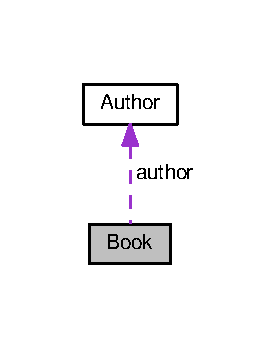
\includegraphics[width=134pt]{classBook__coll__graph}
\end{center}
\end{figure}
\subsection*{Public Member Functions}
\begin{DoxyCompactItemize}
\item 
\hyperlink{classBook_aeaaa3bc96a448032baf5aef373a81d4c}{Book} (const string \&\hyperlink{classBook_a9afedb80b692466dc2d91f109970a32c}{name}, const \hyperlink{classAuthor}{Author} \&\hyperlink{classBook_a1c84f2a0d3db51a0c65f061c91096053}{author}, double \hyperlink{classBook_afa8e149d0bfb4372166d0ccfe8aa30b7}{price}, int \hyperlink{classBook_ae828efa39fa83ff5a8dc3c66e78454e2}{qty\+In\+Stock}=0)
\item 
string \hyperlink{classBook_a1805804b65b05f85adaf94955989e5d0}{get\+Name} () const 
\item 
\hyperlink{classAuthor}{Author} \hyperlink{classBook_a81bfb916599a88e566ebb23162a8c557}{get\+Author} () const 
\item 
double \hyperlink{classBook_a3a3c43b4ab227b3eecba9e414d36c236}{get\+Price} () const 
\item 
void \hyperlink{classBook_a087155b5ee84047d6775b564b92b1778}{set\+Price} (double \hyperlink{classBook_afa8e149d0bfb4372166d0ccfe8aa30b7}{price})
\item 
int \hyperlink{classBook_a123d03e3061f580fefba69b16004954c}{get\+Qty\+In\+Stock} () const 
\item 
void \hyperlink{classBook_ae719f6e8595788d4a6d4126ad073a465}{set\+Qty\+In\+Stock} (int \hyperlink{classBook_ae828efa39fa83ff5a8dc3c66e78454e2}{qty\+In\+Stock})
\item 
void \hyperlink{classBook_a1560f1015348a6d404d1ac069bead1a2}{print} () const 
\item 
string \hyperlink{classBook_ae152ba70b32871377378adf8e87a91ea}{get\+Author\+Name} () const 
\end{DoxyCompactItemize}
\subsection*{Private Attributes}
\begin{DoxyCompactItemize}
\item 
string \hyperlink{classBook_a9afedb80b692466dc2d91f109970a32c}{name}
\item 
\hyperlink{classAuthor}{Author} \hyperlink{classBook_a1c84f2a0d3db51a0c65f061c91096053}{author}
\item 
double \hyperlink{classBook_afa8e149d0bfb4372166d0ccfe8aa30b7}{price}
\item 
int \hyperlink{classBook_ae828efa39fa83ff5a8dc3c66e78454e2}{qty\+In\+Stock}
\end{DoxyCompactItemize}


\subsection{Constructor \& Destructor Documentation}
\index{Book@{Book}!Book@{Book}}
\index{Book@{Book}!Book@{Book}}
\subsubsection[{\texorpdfstring{Book(const string \&name, const Author \&author, double price, int qty\+In\+Stock=0)}{Book(const string &name, const Author &author, double price, int qtyInStock=0)}}]{\setlength{\rightskip}{0pt plus 5cm}Book\+::\+Book (
\begin{DoxyParamCaption}
\item[{const string \&}]{name, }
\item[{const {\bf Author} \&}]{author, }
\item[{double}]{price, }
\item[{int}]{qty\+In\+Stock = {\ttfamily 0}}
\end{DoxyParamCaption}
)}\hypertarget{classBook_aeaaa3bc96a448032baf5aef373a81d4c}{}\label{classBook_aeaaa3bc96a448032baf5aef373a81d4c}

\begin{DoxyCode}
9       : \hyperlink{classBook_a9afedb80b692466dc2d91f109970a32c}{name}(\hyperlink{classBook_a9afedb80b692466dc2d91f109970a32c}{name}), \hyperlink{classBook_a1c84f2a0d3db51a0c65f061c91096053}{author}(author) \{ \textcolor{comment}{// Init object reference in member initializer list}
10    \textcolor{comment}{// Call setters to validate price and qtyInStock}
11    \hyperlink{classBook_a087155b5ee84047d6775b564b92b1778}{setPrice}(\hyperlink{classBook_afa8e149d0bfb4372166d0ccfe8aa30b7}{price});
12    \hyperlink{classBook_ae719f6e8595788d4a6d4126ad073a465}{setQtyInStock}(\hyperlink{classBook_ae828efa39fa83ff5a8dc3c66e78454e2}{qtyInStock});
13 \}
\end{DoxyCode}


Here is the call graph for this function\+:
\nopagebreak
\begin{figure}[H]
\begin{center}
\leavevmode
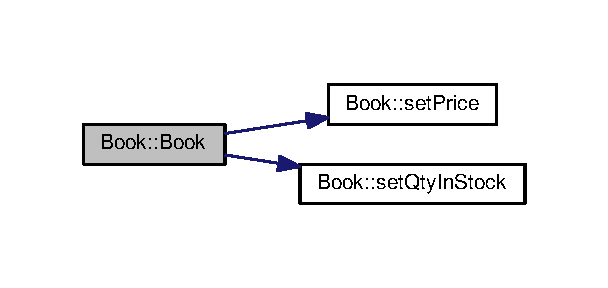
\includegraphics[width=292pt]{classBook_aeaaa3bc96a448032baf5aef373a81d4c_cgraph}
\end{center}
\end{figure}




\subsection{Member Function Documentation}
\index{Book@{Book}!get\+Author@{get\+Author}}
\index{get\+Author@{get\+Author}!Book@{Book}}
\subsubsection[{\texorpdfstring{get\+Author() const }{getAuthor() const }}]{\setlength{\rightskip}{0pt plus 5cm}{\bf Author} Book\+::get\+Author (
\begin{DoxyParamCaption}
{}
\end{DoxyParamCaption}
) const}\hypertarget{classBook_a81bfb916599a88e566ebb23162a8c557}{}\label{classBook_a81bfb916599a88e566ebb23162a8c557}

\begin{DoxyCode}
19                        \{
20    \textcolor{keywordflow}{return} \hyperlink{classBook_a1c84f2a0d3db51a0c65f061c91096053}{author};
21 \}
\end{DoxyCode}
\index{Book@{Book}!get\+Author\+Name@{get\+Author\+Name}}
\index{get\+Author\+Name@{get\+Author\+Name}!Book@{Book}}
\subsubsection[{\texorpdfstring{get\+Author\+Name() const }{getAuthorName() const }}]{\setlength{\rightskip}{0pt plus 5cm}string Book\+::get\+Author\+Name (
\begin{DoxyParamCaption}
{}
\end{DoxyParamCaption}
) const}\hypertarget{classBook_ae152ba70b32871377378adf8e87a91ea}{}\label{classBook_ae152ba70b32871377378adf8e87a91ea}

\begin{DoxyCode}
58                                  \{
59    \textcolor{keywordflow}{return} \hyperlink{classBook_a1c84f2a0d3db51a0c65f061c91096053}{author}.\hyperlink{classAuthor_a2d27943db18f822be1a301bca65fb6ef}{getName}();   \textcolor{comment}{// invoke the getName() on instance author}
60 \}\end{DoxyCode}


Here is the call graph for this function\+:
\nopagebreak
\begin{figure}[H]
\begin{center}
\leavevmode
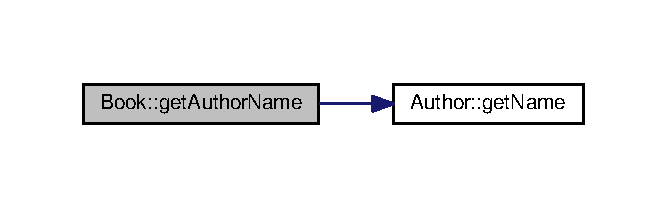
\includegraphics[width=320pt]{classBook_ae152ba70b32871377378adf8e87a91ea_cgraph}
\end{center}
\end{figure}


\index{Book@{Book}!get\+Name@{get\+Name}}
\index{get\+Name@{get\+Name}!Book@{Book}}
\subsubsection[{\texorpdfstring{get\+Name() const }{getName() const }}]{\setlength{\rightskip}{0pt plus 5cm}string Book\+::get\+Name (
\begin{DoxyParamCaption}
{}
\end{DoxyParamCaption}
) const}\hypertarget{classBook_a1805804b65b05f85adaf94955989e5d0}{}\label{classBook_a1805804b65b05f85adaf94955989e5d0}

\begin{DoxyCode}
15                            \{
16    \textcolor{keywordflow}{return} \hyperlink{classBook_a9afedb80b692466dc2d91f109970a32c}{name};
17 \}
\end{DoxyCode}
\index{Book@{Book}!get\+Price@{get\+Price}}
\index{get\+Price@{get\+Price}!Book@{Book}}
\subsubsection[{\texorpdfstring{get\+Price() const }{getPrice() const }}]{\setlength{\rightskip}{0pt plus 5cm}double Book\+::get\+Price (
\begin{DoxyParamCaption}
{}
\end{DoxyParamCaption}
) const}\hypertarget{classBook_a3a3c43b4ab227b3eecba9e414d36c236}{}\label{classBook_a3a3c43b4ab227b3eecba9e414d36c236}

\begin{DoxyCode}
23                             \{
24    \textcolor{keywordflow}{return} \hyperlink{classBook_afa8e149d0bfb4372166d0ccfe8aa30b7}{price};
25 \}
\end{DoxyCode}
\index{Book@{Book}!get\+Qty\+In\+Stock@{get\+Qty\+In\+Stock}}
\index{get\+Qty\+In\+Stock@{get\+Qty\+In\+Stock}!Book@{Book}}
\subsubsection[{\texorpdfstring{get\+Qty\+In\+Stock() const }{getQtyInStock() const }}]{\setlength{\rightskip}{0pt plus 5cm}int Book\+::get\+Qty\+In\+Stock (
\begin{DoxyParamCaption}
{}
\end{DoxyParamCaption}
) const}\hypertarget{classBook_a123d03e3061f580fefba69b16004954c}{}\label{classBook_a123d03e3061f580fefba69b16004954c}

\begin{DoxyCode}
37                               \{
38    \textcolor{keywordflow}{return} \hyperlink{classBook_ae828efa39fa83ff5a8dc3c66e78454e2}{qtyInStock};
39 \}
\end{DoxyCode}
\index{Book@{Book}!print@{print}}
\index{print@{print}!Book@{Book}}
\subsubsection[{\texorpdfstring{print() const }{print() const }}]{\setlength{\rightskip}{0pt plus 5cm}void Book\+::print (
\begin{DoxyParamCaption}
{}
\end{DoxyParamCaption}
) const}\hypertarget{classBook_a1560f1015348a6d404d1ac069bead1a2}{}\label{classBook_a1560f1015348a6d404d1ac069bead1a2}

\begin{DoxyCode}
52                        \{
53    cout << \textcolor{stringliteral}{"'"} << \hyperlink{classBook_a9afedb80b692466dc2d91f109970a32c}{name} << \textcolor{stringliteral}{"' by "};
54    \hyperlink{classBook_a1c84f2a0d3db51a0c65f061c91096053}{author}.\hyperlink{classAuthor_a5d5d6296cd6cf5c5017fc2f27a8f6925}{print}();
55 \}
\end{DoxyCode}


Here is the call graph for this function\+:
\nopagebreak
\begin{figure}[H]
\begin{center}
\leavevmode
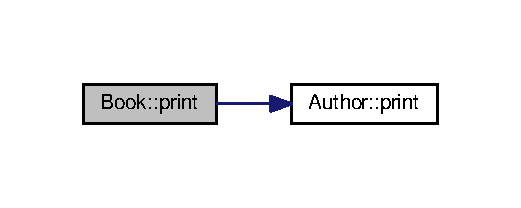
\includegraphics[width=250pt]{classBook_a1560f1015348a6d404d1ac069bead1a2_cgraph}
\end{center}
\end{figure}


\index{Book@{Book}!set\+Price@{set\+Price}}
\index{set\+Price@{set\+Price}!Book@{Book}}
\subsubsection[{\texorpdfstring{set\+Price(double price)}{setPrice(double price)}}]{\setlength{\rightskip}{0pt plus 5cm}void Book\+::set\+Price (
\begin{DoxyParamCaption}
\item[{double}]{price}
\end{DoxyParamCaption}
)}\hypertarget{classBook_a087155b5ee84047d6775b564b92b1778}{}\label{classBook_a087155b5ee84047d6775b564b92b1778}

\begin{DoxyCode}
28                                 \{
29    \textcolor{keywordflow}{if} (\hyperlink{classBook_afa8e149d0bfb4372166d0ccfe8aa30b7}{price} > 0) \{
30       this->\hyperlink{classBook_afa8e149d0bfb4372166d0ccfe8aa30b7}{price} = \hyperlink{classBook_afa8e149d0bfb4372166d0ccfe8aa30b7}{price};
31    \} \textcolor{keywordflow}{else} \{
32       cout << \textcolor{stringliteral}{"price should be positive! Set to 0"} << endl;
33       this->\hyperlink{classBook_afa8e149d0bfb4372166d0ccfe8aa30b7}{price} = 0;
34    \}
35 \}
\end{DoxyCode}
\index{Book@{Book}!set\+Qty\+In\+Stock@{set\+Qty\+In\+Stock}}
\index{set\+Qty\+In\+Stock@{set\+Qty\+In\+Stock}!Book@{Book}}
\subsubsection[{\texorpdfstring{set\+Qty\+In\+Stock(int qty\+In\+Stock)}{setQtyInStock(int qtyInStock)}}]{\setlength{\rightskip}{0pt plus 5cm}void Book\+::set\+Qty\+In\+Stock (
\begin{DoxyParamCaption}
\item[{int}]{qty\+In\+Stock}
\end{DoxyParamCaption}
)}\hypertarget{classBook_ae719f6e8595788d4a6d4126ad073a465}{}\label{classBook_ae719f6e8595788d4a6d4126ad073a465}

\begin{DoxyCode}
42                                        \{
43    \textcolor{keywordflow}{if} (\hyperlink{classBook_ae828efa39fa83ff5a8dc3c66e78454e2}{qtyInStock} >= 0) \{
44       this->\hyperlink{classBook_ae828efa39fa83ff5a8dc3c66e78454e2}{qtyInStock} = \hyperlink{classBook_ae828efa39fa83ff5a8dc3c66e78454e2}{qtyInStock};
45    \} \textcolor{keywordflow}{else} \{
46       cout << \textcolor{stringliteral}{"qtyInStock cannnot be negative! Set to 0"} << endl;
47       this->\hyperlink{classBook_ae828efa39fa83ff5a8dc3c66e78454e2}{qtyInStock} = 0;
48    \}
49 \}
\end{DoxyCode}


\subsection{Member Data Documentation}
\index{Book@{Book}!author@{author}}
\index{author@{author}!Book@{Book}}
\subsubsection[{\texorpdfstring{author}{author}}]{\setlength{\rightskip}{0pt plus 5cm}{\bf Author} Book\+::author\hspace{0.3cm}{\ttfamily [private]}}\hypertarget{classBook_a1c84f2a0d3db51a0c65f061c91096053}{}\label{classBook_a1c84f2a0d3db51a0c65f061c91096053}
\index{Book@{Book}!name@{name}}
\index{name@{name}!Book@{Book}}
\subsubsection[{\texorpdfstring{name}{name}}]{\setlength{\rightskip}{0pt plus 5cm}string Book\+::name\hspace{0.3cm}{\ttfamily [private]}}\hypertarget{classBook_a9afedb80b692466dc2d91f109970a32c}{}\label{classBook_a9afedb80b692466dc2d91f109970a32c}
\index{Book@{Book}!price@{price}}
\index{price@{price}!Book@{Book}}
\subsubsection[{\texorpdfstring{price}{price}}]{\setlength{\rightskip}{0pt plus 5cm}double Book\+::price\hspace{0.3cm}{\ttfamily [private]}}\hypertarget{classBook_afa8e149d0bfb4372166d0ccfe8aa30b7}{}\label{classBook_afa8e149d0bfb4372166d0ccfe8aa30b7}
\index{Book@{Book}!qty\+In\+Stock@{qty\+In\+Stock}}
\index{qty\+In\+Stock@{qty\+In\+Stock}!Book@{Book}}
\subsubsection[{\texorpdfstring{qty\+In\+Stock}{qtyInStock}}]{\setlength{\rightskip}{0pt plus 5cm}int Book\+::qty\+In\+Stock\hspace{0.3cm}{\ttfamily [private]}}\hypertarget{classBook_ae828efa39fa83ff5a8dc3c66e78454e2}{}\label{classBook_ae828efa39fa83ff5a8dc3c66e78454e2}


The documentation for this class was generated from the following files\+:\begin{DoxyCompactItemize}
\item 
\hyperlink{Book_8h}{Book.\+h}\item 
\hyperlink{Book_8cpp}{Book.\+cpp}\end{DoxyCompactItemize}

\chapter{File Documentation}
\hypertarget{Author_8cpp}{}\section{Author.\+cpp File Reference}
\label{Author_8cpp}\index{Author.\+cpp@{Author.\+cpp}}
{\ttfamily \#include $<$iostream$>$}\\*
{\ttfamily \#include \char`\"{}Author.\+h\char`\"{}}\\*
Include dependency graph for Author.\+cpp\+:
\nopagebreak
\begin{figure}[H]
\begin{center}
\leavevmode
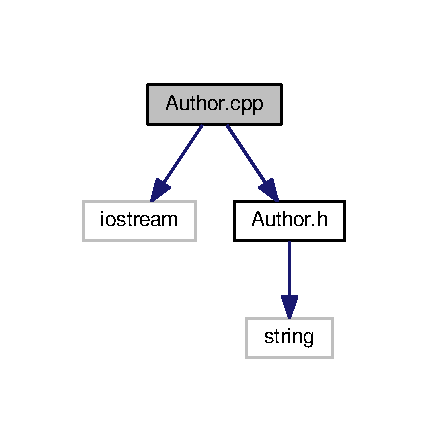
\includegraphics[width=206pt]{Author_8cpp__incl}
\end{center}
\end{figure}

\hypertarget{Author_8h}{}\section{Author.\+h File Reference}
\label{Author_8h}\index{Author.\+h@{Author.\+h}}
{\ttfamily \#include $<$string$>$}\\*
Include dependency graph for Author.\+h\+:
\nopagebreak
\begin{figure}[H]
\begin{center}
\leavevmode
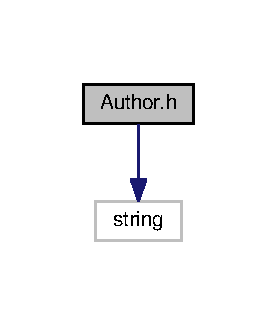
\includegraphics[width=133pt]{Author_8h__incl}
\end{center}
\end{figure}
This graph shows which files directly or indirectly include this file\+:
\nopagebreak
\begin{figure}[H]
\begin{center}
\leavevmode
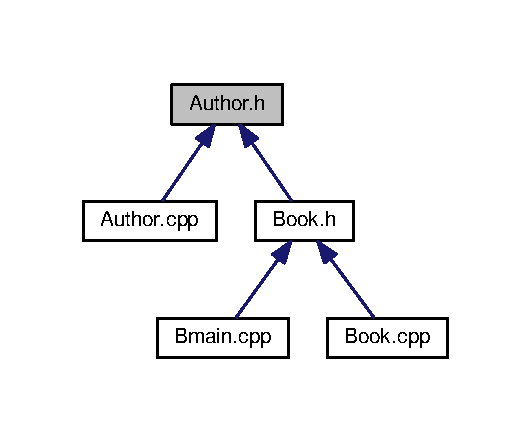
\includegraphics[width=255pt]{Author_8h__dep__incl}
\end{center}
\end{figure}
\subsection*{Classes}
\begin{DoxyCompactItemize}
\item 
class \hyperlink{classAuthor}{Author}
\end{DoxyCompactItemize}

\hypertarget{Bmain_8cpp}{}\section{Bmain.\+cpp File Reference}
\label{Bmain_8cpp}\index{Bmain.\+cpp@{Bmain.\+cpp}}
{\ttfamily \#include $<$iostream$>$}\\*
{\ttfamily \#include \char`\"{}Ball.\+h\char`\"{}}\\*
Include dependency graph for Bmain.\+cpp\+:
\nopagebreak
\begin{figure}[H]
\begin{center}
\leavevmode
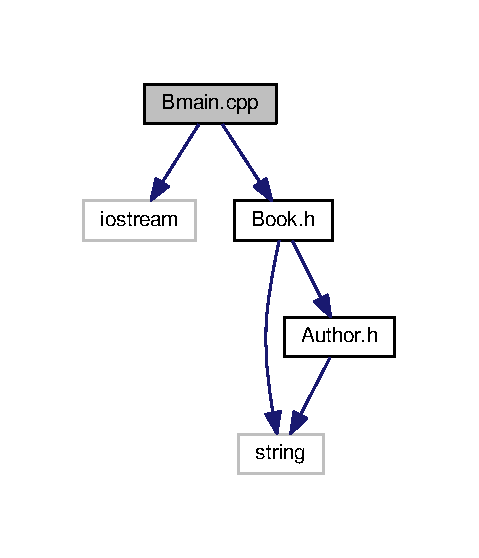
\includegraphics[width=194pt]{Bmain_8cpp__incl}
\end{center}
\end{figure}
\subsection*{Functions}
\begin{DoxyCompactItemize}
\item 
int \hyperlink{Bmain_8cpp_ae66f6b31b5ad750f1fe042a706a4e3d4}{main} ()
\end{DoxyCompactItemize}


\subsection{Function Documentation}
\index{Bmain.\+cpp@{Bmain.\+cpp}!main@{main}}
\index{main@{main}!Bmain.\+cpp@{Bmain.\+cpp}}
\subsubsection[{\texorpdfstring{main()}{main()}}]{\setlength{\rightskip}{0pt plus 5cm}int main (
\begin{DoxyParamCaption}
{}
\end{DoxyParamCaption}
)}\hypertarget{Bmain_8cpp_ae66f6b31b5ad750f1fe042a706a4e3d4}{}\label{Bmain_8cpp_ae66f6b31b5ad750f1fe042a706a4e3d4}

\begin{DoxyCode}
6            \{
7    \hyperlink{classBall}{Ball} ball;
8    ball.\hyperlink{classBall_afb29247bbe8aa061a1212a0bd3d7c4b8}{print}();    \textcolor{comment}{// Ball @ (0.00,0.00) with speed (0.00,0.00)}
9    ball.\hyperlink{classBall_af38e5a6a3556b833cff90c2cd5292713}{setXY}(1.1, 2.2);
10    ball.\hyperlink{classBall_a1063b6a3532786b7147fad5e07182a45}{setXYSpeed}(3.3, 4.4);
11    ball.\hyperlink{classBall_afb29247bbe8aa061a1212a0bd3d7c4b8}{print}();    \textcolor{comment}{// Ball @ (1.10,2.20) with speed (3.30,4.40)}
12    ball.\hyperlink{classBall_a5499dc9c66f5f79c535ca970b02a9cee}{setX}(5.5);
13    ball.\hyperlink{classBall_a3216c6c42326d379f4a884993bea7e70}{setY}(6.6);
14    cout << \textcolor{stringliteral}{"x is "} << ball.\hyperlink{classBall_a480a1d4547fea337598d6d5b7fb83d8f}{getX}() << endl;  \textcolor{comment}{// x is 5.50}
15    cout << \textcolor{stringliteral}{"y is "} << ball.\hyperlink{classBall_a28a7fe3223d2c192e0eefaa75074e820}{getY}() << endl;  \textcolor{comment}{// y is 6.60}
16    ball.\hyperlink{classBall_a05228e822d67b25baf715cf09c325494}{move}();
17    ball.\hyperlink{classBall_afb29247bbe8aa061a1212a0bd3d7c4b8}{print}();    \textcolor{comment}{// Ball @ (8.80,11.00) with speed (3.30,4.40)}
18 \}\end{DoxyCode}


Here is the call graph for this function\+:
\nopagebreak
\begin{figure}[H]
\begin{center}
\leavevmode
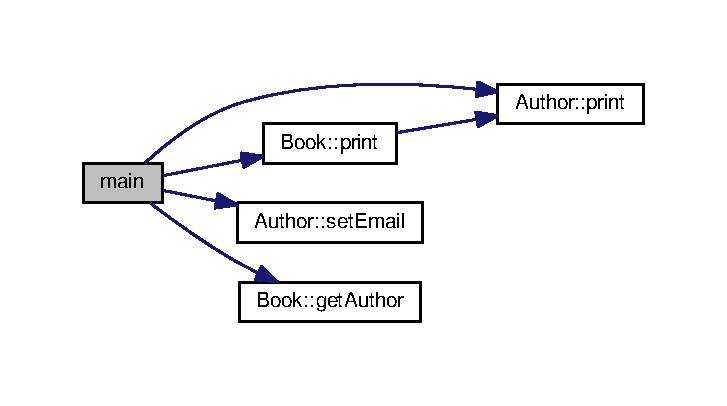
\includegraphics[width=350pt]{Bmain_8cpp_ae66f6b31b5ad750f1fe042a706a4e3d4_cgraph}
\end{center}
\end{figure}



\hypertarget{Book_8cpp}{}\section{Book.\+cpp File Reference}
\label{Book_8cpp}\index{Book.\+cpp@{Book.\+cpp}}
{\ttfamily \#include $<$iostream$>$}\\*
{\ttfamily \#include \char`\"{}Book.\+h\char`\"{}}\\*
Include dependency graph for Book.\+cpp\+:
\nopagebreak
\begin{figure}[H]
\begin{center}
\leavevmode
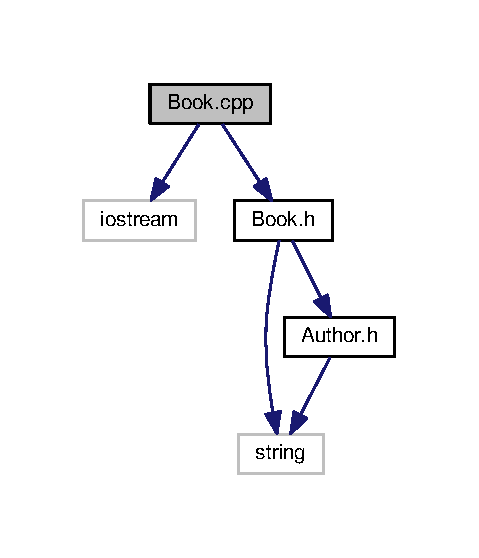
\includegraphics[width=230pt]{Book_8cpp__incl}
\end{center}
\end{figure}

\hypertarget{Book_8h}{}\section{Book.\+h File Reference}
\label{Book_8h}\index{Book.\+h@{Book.\+h}}
{\ttfamily \#include $<$string$>$}\\*
{\ttfamily \#include \char`\"{}Author.\+h\char`\"{}}\\*
Include dependency graph for Book.\+h\+:
\nopagebreak
\begin{figure}[H]
\begin{center}
\leavevmode
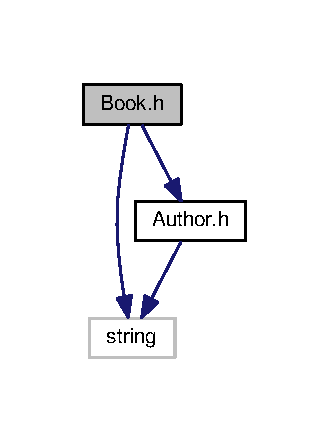
\includegraphics[width=158pt]{Book_8h__incl}
\end{center}
\end{figure}
This graph shows which files directly or indirectly include this file\+:
\nopagebreak
\begin{figure}[H]
\begin{center}
\leavevmode
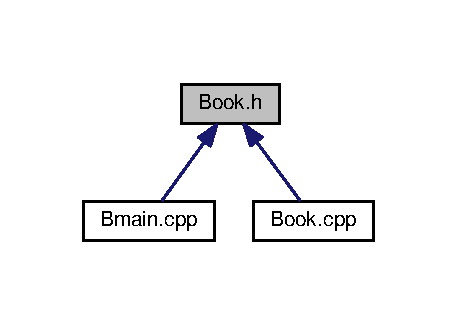
\includegraphics[width=220pt]{Book_8h__dep__incl}
\end{center}
\end{figure}
\subsection*{Classes}
\begin{DoxyCompactItemize}
\item 
class \hyperlink{classBook}{Book}
\end{DoxyCompactItemize}

%--- End generated contents ---

% Index
\backmatter
\newpage
\phantomsection
\clearemptydoublepage
\addcontentsline{toc}{chapter}{Index}
\printindex

\end{document}
